\documentclass[10pt]{article}
\usepackage[margin=0.72in]{geometry}
\usepackage{graphicx,booktabs,hyperref}
\hypersetup{colorlinks=true,urlcolor=blue}
\title{Point-driven pencil collector: completed small-size cohorts}
\author{Reproducible experiment report}
\date{21 October 2026}
\begin{document}
\maketitle
\noindent\textbf{Scope.} Seven exact-order Scholten models, 60 public targets
per model: one 16-bit, three 20-bit and three 24-bit source subgroups. Every
candidate and same-process source-negation-rho scalar was recomputed on the
source curve by the producer. The independent replay and source validator has
completed all 420 targets across the seven raw files.
The full 21-model, 1,260-target requirement is still open. This document
reports measured counts, not a conclusion for the unrun sizes.

\section*{Observed full one-target costs}
Each pencil solve includes rational-point enumeration, transfer and subgroup
checks, point-driven sieve, Jacobian verification, sparse modular elimination,
and source verification. The curve setup was physically reused for the 60
targets but its entire measured cost is charged to every cold one-target
solve. At $M+0.5S+10I$ and 0.1 source-addition equivalents (GAE) per native
logical operation:
\begin{center}\small
\begin{tabular}{rrrrr}
\toprule
$p$ & Verified targets & Verified relations & Row updates & Pencil/rho \\
\midrule
739 & 60/60 & 21,550 & 6,288,519 & 12.931178 \\
3,371 & 60/60 & 98,666 & 442,470,426 & 246.117110 \\
3,527 & 60/60 & 103,256 & 499,795,794 & 267.374941 \\
3,931 & 60/60 & 114,989 & 690,243,338 & 332.187349 \\
11,731 & 60/60 & 343,641 & 17,235,887,587 & 4,331.361006 \\
11,887 & 60/60 & 348,343 & 17,655,108,982 & 3,856.238613 \\
12,143 & 60/60 & 355,615 & 19,113,208,311 & 4,250.094923 \\
\bottomrule
\end{tabular}
\end{center}

\begin{center}
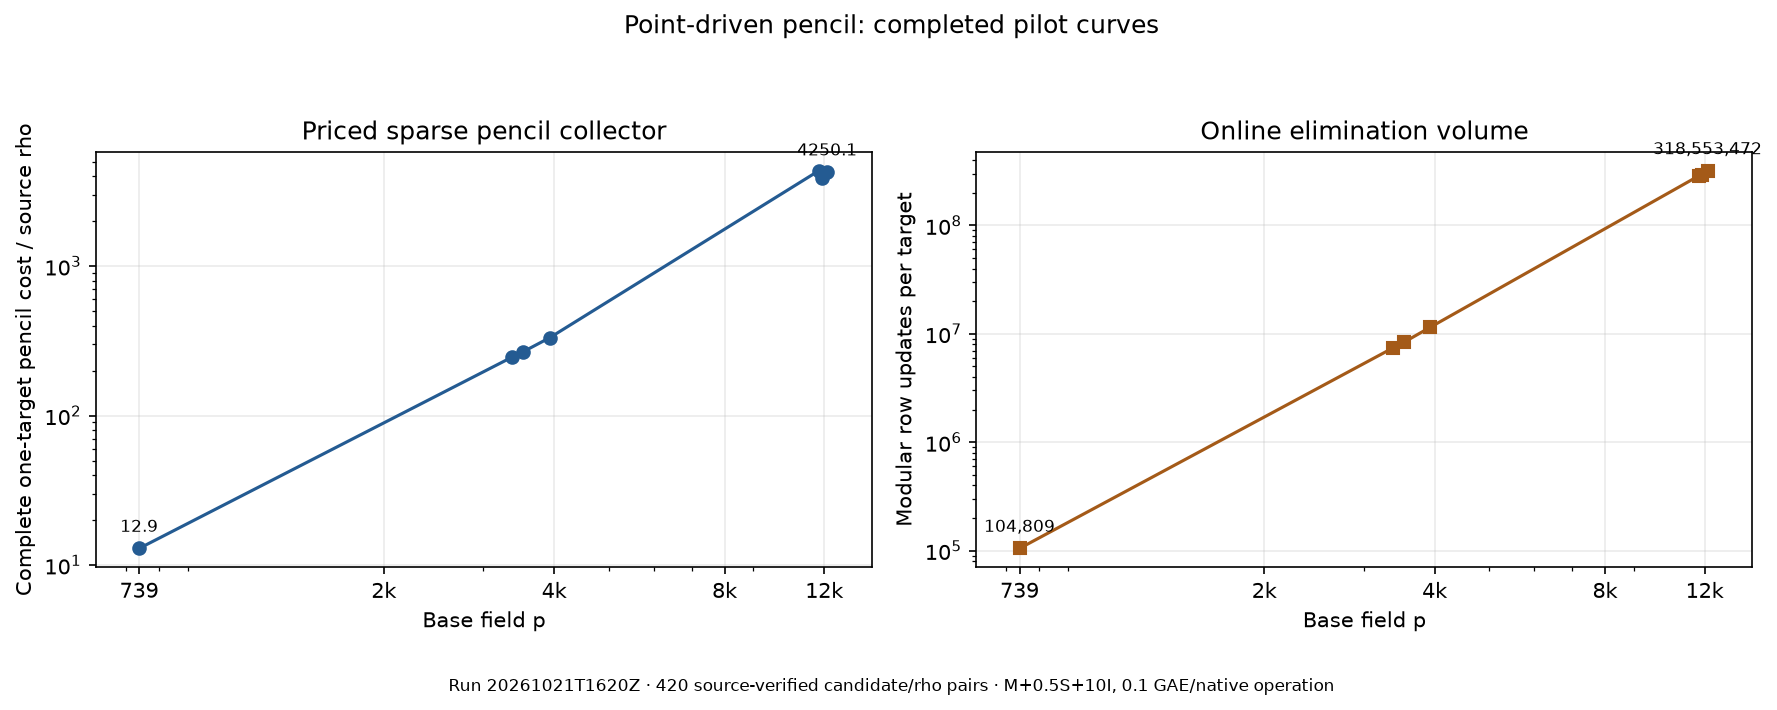
\includegraphics[width=0.85\linewidth]{pencil-pilot-cost.png}
\end{center}

\noindent\textbf{Accounting.} The direct prime-field modular arithmetic is
recorded separately from the Jacobian backend. For each base-field inversion
call, multiplications internal to its Fermat exponentiation are removed from
the direct-multiplication count when the $I$ price is applied; scalar modular
arithmetic and one sparse-map update per recorded row update are charged at
the declared native rate. All 36 pricing cells per model are in
\path{results/pencil-pilot/price-grid.csv}. The same-process rho counts and
native counters match the earlier frozen rho controls on every target.

The F739 port reproduces all 61 earlier setup/target records after removing
wall-clock fields. The sparse-row collector then recovered all 420 public
scalars across these seven models. The raw JSONL and Rust analyzer are under
\path{results/pencil-pilot/} and \path{src/bin/analyze_pencil.rs}. One
algorithm seed per target was used; no uncertainty interval or qualified
wall-speed measurement was made.
\end{document}
